\documentclass[12pt,english]{article}
\usepackage[utf8]{inputenc}
\usepackage{tgpagella} % Palatino text only
\usepackage{mathpazo}  % Palatino math & text
\usepackage[left=1.5in,right=1.5in,top=1.5in,bottom=1.5in]{geometry}
% \linespread{1.5}
% \usepackage[super,comma,sort]{natbib}
\usepackage[round,sort&compress]{natbib}
\usepackage{url} % [hyphens]
\usepackage[hyperpageref]{backref} % back references biblio. Needs latexmk at compilation.
\usepackage[pagebackref]{hyperref}
% \usepackage{multibib} % incompatible with backref
\hypersetup{
  colorlinks=true, % breaklinks=true,
  urlcolor=purple,    % color of external links
  linkcolor=blue,  % color of toc, list of figs etc.
  citecolor=violet,   % color of links to bibliography
}
\usepackage{bm}
\usepackage{indentfirst}
\usepackage{tocbibind}
\setcitestyle{aysep={}} 
\usepackage{amsmath}
\usepackage{amssymb}
\usepackage{eurosym}
\usepackage{amsfonts}
\usepackage{enumerate}
\usepackage{babel}
\usepackage{caption}
\usepackage{supertabular}
\usepackage{tabularx}
\usepackage{float}
\usepackage{dsfont}
\usepackage{fancyvrb}
\usepackage{verbatim}
\usepackage{enumitem}
\usepackage{setspace}
\usepackage{comment}
\usepackage{subcaption}
\usepackage{graphicx}
\usepackage{tikz}
\usepackage{gensymb}
\usepackage{textcomp}

\usepackage{tabulary}
\usepackage{tabularx}
\usepackage{booktabs}
\usepackage{fullpage}
\usepackage{morefloats}
\usepackage{makecell}
\usepackage{lscape}
\usepackage{pdflscape}
\usepackage{longtable}
\usepackage{rotating}
\usepackage{fancyhdr}
\usepackage{tocloft}
\usepackage{titletoc}
\usepackage[export]{adjustbox}
\usepackage[anythingbreaks]{breakurl} % for links
\usepackage{multicol}
\newsavebox\ltmcbox % For net gain table over two columns
%\usepackage[nomarkers,figuresonly]{endfloat} % Figures at the end
%\usepackage[section,below]{placeins} % Floats placed in the section they appear in.
\renewcommand{\floatpagefraction}{.9}

\title{A Global Wealth Tax -- Policy Brief
} 

% \author{Global Redistribution Advocates\footnote{The author is Adrien Fabre, CNRS researcher in economics at CIRED. E-mail: fabre.adri1@gmail.com.}} 
\author{\textcolor{white}{Adrien Fabre\footnote{\textcolor{black}{The author is Adrien Fabre, CNRS researcher in economics at CIRED. E-mail: adrien.fabre@cnrs.fr.}}}
%\footnote{CNRS researcher in economics at CIRED. E-mail: adrien.fabre@cnrs.fr.}
} 
% \author{Global Redistribution Advocates\footnote{The author is Adrien Fabre, CNRS researcher in economics at CIRED. E-mail: fabre.adri1@gmail.com.}} 

\date{\today{} -- \href{https://github.com/bixiou/global_tax_attitudes/raw/main/paper/policy_brief_tax.pdf}{Link to most recent version}} 

\begin{document}
% TODO! add conditionality on social protection

\maketitle
\tikz [remember picture, overlay] %
\node [shift={(5.5cm,-1.5cm)}] at (current page.north west) % north west
[anchor=north west] % north west
{\href{http://global-redistribution-advocates.org}{
\includegraphics[height=1.3cm]{../figures/policies/logo_full_white_bg}}};

\begin{center}
{\textbf{\href{https://github.com/bixiou/global_tax_attitudes/raw/main/paper/policy_brief_tax.pdf}{Link to most recent version}}}
\end{center}

\begin{figure}[h!]
  \caption{Support for a Global Wealth Tax (in percent).}\label{fig:support}
  \makebox[\textwidth][c]{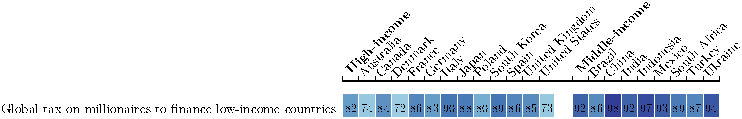
\includegraphics[width=1.2\textwidth]{../figures/OECD/Heatplot_global_tax_attitudes_tax_share.pdf}} 
\end{figure}


\section{Summary}\label{sec:intro}

\citet{fabre_international_2023} survey attitudes toward global policies in 20 among the largest countries and find near consensus for a global tax on millionaires that would finance low-income countries. The world's richest 1\% (those with a wealth above \euro{}900,000) own 38\% of global wealth \citep{chancel_world_2022}, and the wealth in excess of \euro{}1 million represents 24\% of global wealth. It is logical that the other 99\% massively support taxing the wealthiest. What is more interesting, 90\% of Americans and 92\% of Europeans want to pool at least 10\% of the revenues of a global wealth tax to finance low-income countries. When asked the preferred amount that should finance low-income countries, the average answer is one third.

In this policy brief, we propose a global wealth tax and specify how its revenues should be allocated between countries (Section \ref{sec:design}), we estimate the distributive effects of such a tax (Section \ref{sec:distribution}), and show that it would be strongly supported all over the world (Section \ref{sec:support}).

\section{Design}\label{sec:design}

\paragraph{Coordinated national wealth taxes.} While action at a global level reduces tax avoidance, taxing wealth at the national level already makes a significant dent on inequality and generates important revenues. 
The implementation of national wealth taxes should therefore not be delayed by the wait of a global wealth tax. 
We call like-minded political parties of all countries to include a wealth tax proposal in their platform, and implement it when they arrive in power. We propose below a design of wealth tax that can be replicated in any country so that national wealth taxes would be compatible and part of a global wealth tax system. 

\paragraph{A progressive tax schedule.} %We define wealth as net wealth, i.e. all assets (financial, real estate, art...) net of debt. %  Saez & Zucman (19, footnote p. 13) reveal that debt is 6% for the top 0.1% (>32M)
% A 2\% tax on wealth in excess of \$5 million would raise \$816 billion each year, that is 0.85\% of the Gross World Product (GWP), half of it coming from the U.S. and less than \$1 billion from all low-income countries (28 countries home to 700 million people) combined. 
% Oxfam has a very close tax schedule: 2% > 5M, 3% > 50M, 5% > 1G. WID simulator says this would raise 1.19% GWP i.e. $1.15T given GWP of 96.5T (vs. 1.3% for our schedule), though Oxfam claims it would raise $1.7 trillion/year, i.e. 1.8% GWP.
Let us introduce a basic example of what a moderate wealth tax can raise, we call it the ``basic'' tax schedule. It consists of a 2\% tax on wealth in excess of \$5 million, a 6\% marginal tax rate above \$100 million, and 10\% above \$1 billion. This basic tax would raise \$1.85 trillion each year, that is 1.76\% of the Gross World Product (GWP). %, half of it coming from the U.S. and less than \$1 billion from all low-income countries (28 countries home to 700 million people) combined. 
% 1-2-3: \$1.37 trillion each year, that is 1.30\% of the Gross World Product (GWP).
% 1.85T comes from WID (which has GWP=105.28T) but World Bank has GWP22=100.56T
\citet{chancel_world_2022} offer a \href{https://wid.world/world-wealth-tax-simulator/}{world wealth tax simulator} that allows estimating the revenues of a custom global wealth tax by world region.\footnote{Similar simulators exist for \href{https://taxjusticenow.org/}{the U.S.} \citep{saez_triumph_2019} and \href{http://taxsimulator.ukwealth.tax/\#/appendix}{the UK} while \citet{kapeller_european_2021} and \citet{oxfam_taxing_2022} offer similar estimates for the EU and many countries, respectively. Despite differences in some assumptions and the data used, all these simulators and calculations yield comparable estimates.} 
For example, a progressive wealth tax with the following schedule could raise 6\% of the GWP: 0.5\% marginal tax rate between \$500,000 and \$1 million, 1\% between \$1 and \$2 million, 3\% between \$2 and \$5 million, 5\% between \$5 and \$20 million, 10\% between \$20 and \$100 million, and 20\% above \$100 million. % TODO: put in table format 
% (according to https://thomasblanchet.github.io/wealth-tax/ for the U.S., 16% GDP short term and 3.7% long-term/ 6% long-term with lump-sum rebate)
% also 6% GWP: 0.5% > 100k; 2% > 500k; 4% > 1M; 5% > 5M; 7% > 20M; 10% > 100M  (according to https://thomasblanchet.github.io/wealth-tax/ for the U.S., 19% GDP short term and 4.3% long-term / 7.6% long-term with lump-sum rebate)
% also 6% GWP: 5% > 500k (according to https://thomasblanchet.github.io/wealth-tax/ for the U.S., 19% GDP short term and 4.1% long-term / 7% long-term with lump-sum rebate)
% Saez & Zucman (19) do so and find 6.25% (in the U.S.) "the long-run revenue-maximizing (annual) wealth tax would be around 6.25 percent". This is from a simple theoretical model with a linear tax on billionaires. In practice, they find that the wealth share of the 400 richest billionaires would have remained constant with a 2% tax >50% and 10% >10G, meaning that that "radical tax" would be close to the revenue-maximizing one. Though in the conclusion they say that it's around 2% that we get no wealth deconcentration, i.e. perennial revenues.
% Blanchet (22) finds a revenue-maximizing rate of 12% above 50M in the U.S.
% In the annex of Piketty's Capital & Ideology (p. 36), he has a back-of-the-envelope calculation (with noseguess hypotheses) of perennial revenues of his wealth tax: 4% of national income (actually in his examples for the U.S. and Europe, he finds at least 6%).
6\% of the GWP is also a good estimate of the long-term revenues that can be reasonably expected from a strongly progressive global wealth tax,\footnote{The last tax schedule applied to the U.S. and rebated equally to all Americans would raise 6\% of the U.S. in the long term according to the \href{https://thomasblanchet.github.io/wealth-tax/}{simulator} of \citet{blanchet_uncovering_2022}, and a similar fraction can be raised at the global level using an appropriate tax schedule.} though more can be collected in the short term with an even more progressive tax (see e.g. \citealp{chancel_world_2022} who propose a top marginal rate of 90\%). 
Ideally, the tax schedule should be defined by democratically aggregating people's preferences \citep{fabre_french_2022}. 
% We propose a minimal rate at 2% and a custom schedule by country, for which the second schedule given seems a reasonable proposal.
% Half of the minimal tax, that is 1\% for wealth in excess of 5M, should be pooled to finance LIC.

\paragraph{A minimum tax to finance lower-income countries.} We propose that all countries introduce the \textit{basic tax schedule} as a minimum wealth tax, and then top it up with the progressive wealth tax of their choice, such as the one just described. 
Half of the basic tax %(that is, a 1\% tax on wealth in excess of \$5 million, a 2\% marginal tax rate above \$100 million, and 3\% above \$1 billion) 
should be pooled and transferred to lower-income countries. More could be pooled, at the discretion of each country. %The United Nations Economic and Social Council (ECOSOC) 
An ad hoc Fund would collect the pooled revenues and allocate them to lower-income countries' governments. This Fund could decide to manage a country's revenues directly if the government seriously violates of human rights or would divert a substantial fraction of the revenues. In such cases, projects and public services would be financed by the Fund and supervised by multilateral development agencies. 

\paragraph{Allocating the revenues in function of the GDP per capita.} The revenues should be allocated in priority to the poorest countries. A good indicator of poverty is the poverty gap: it expresses the minimum amount that would be required to lift everyone above the poverty line. However, allocating revenues in function of the poverty gap would disincentivize countries' governments to effectivly address poverty. To avoid bad incentives, it is preferrable to allocate the revenues in function of a well-measured indicator correlated to the poverty gap. We propose an allocation key based on GDP per capita, according to how it predicts the poverty gap predicted in a linear regression (see more details below). 

% 1% above 5M for low-income countries + countries are free to top up that with a more progressive wealth tax. Examples of rates and revenues per country.
% revenues allocation

% Proposal of Piketty in last chapter of Capital and Ideology: 0.1% above 0.5 of average wealth i.e. 37k; 1% > 2 = 150k; 2% > 5 = 370k; 5% > 10 = 740k; 10% > 100 = 7.4M; 60% > 1k = 74M; 90% > 10k = 740M
% Mean global wealth: €74k
% Most progressive scenario in WIR (22): 1% > 1M; 1.5% > 10M; 7% > 100M; 15% > 1G; 50% > 10G; 90% > 100G


% \~ 50M millionaires \~ top 1\% \~ 1/3 wealth \~ 3M/millionaire \~ 150T\$ (Table 4.1 (p. 90) de World Inequality Report 2022)
% => Progressive millionaire tax can yield max 5-7T\$/year i.e. 5-7\% of world GDP.
% Tax at 1\% above 1M, 2\% > 2M, 3\% > 5M, 5\% > 20M, 10\% > 100M yield 3.2\% of world GDP.
% Tax at 2\% above 5M, 5\% > 20M, 7\% > 100M yield 1.9\% of world GDP. https://wid.world/world-wealth-tax-simulator/

% China has probably around 1/6 of millionaire wealth, i.e. 1\% of world GDP from max tax. 
% China's exported emissions is probably around 6\% of world total. Counting 1.7\% of world GDP in ETS revenues, that's 0.1\% of world GDP for China's exported emissions.
\section{Distributive effects}\label{sec:distribution}

\paragraph{Taxing the global top 1\%.} To fully specify its distributive effects, we would need to know what the wealth tax would finance. As it can be used to finance a range of programs which benefit different people, the only precise estimates we can give relate to the losers of the policy: the wealthiest people who would be taxed. The basic tax would only affect people with a wealth above \$5 million, which represent less than 0.1\% of the world adult population (0.7\% of the population in the U.S. and Canada, and 0.2\% in Europe). A tax on all millionaires (in dollars) would affect 1.2\% of adults worldwide (7\% in the U.S. and Canada, 3\% in Europe). While we do not detail the distributive effects between individuals, we describe the distributive effects between countries.

% 1.76
\paragraph{1\% of the Global World Product redistributed to lower income countries.} Assuming that countries do not pool for low-income countries more revenues than half of the basic tax, the redistribution between countries is financed by a 1\% tax on wealth in excess of \$5 million, a 3\% marginal tax rate above \$100 million, and 5\% above \$1 billion. Such a tax would raise 0.9\% of the Gross World Product, that is \$926 %1-2-3: 687 % 447
billion per year.\footnote{The calculations were realized using the \href{https://wid.world/world-wealth-tax-simulator/}{world wealth tax simulator}.} The tax would raise \$392 billion from the U.S. and Canada (that is 2.11\% of their GDP), 
%nearly half of its revenues from the U.S. and Canada (\$198 billion, i.e. 1.07\% of their GDP), 
\$221 billion from East Asia (0.73\%), \$172 billion from Europe (1.00\%), \$51 billion from South and South East Asia (0.32\%), \$36 billion from Latin America (0.49\%), \$27 billion from the Middle East and North Africa (0.35\%), \$20 billion from Russia and Central Asia (0.46\%), and \$5 billion from Sub-Saharan Africa (0.14\%). 
% 1-2-3: The tax would raise \$296 billion from the U.S. and Canada (that is 1.59\% of their GDP), 
%nearly half of its revenues from the U.S. and Canada (\$198 billion, i.e. 1.07\% of their GDP), \$162 billion from East Asia (0.54\%), \$127 billion from Europe (0.74\%), \$35 billion from South and South East Asia (0.22\%), \$27 billion from Latin America (0.38\%), \$21 billion from the Middle East and North Africa (0.27\%), \$13 billion from Russia and Central Asia (0.30\%), and \$4 billion from Sub-Saharan Africa (0.11\%). 
% \$198 billion from the U.S. and Canada (that is 1.59\% of their GDP), \$103 billion from East Asia (0.34\%), \$83 billion from Europe (0.48\%), \$19 billion from South and South East Asia (0.12\%), \$16 billion from the Middle East and North Africa (0.20\%), \$6 billion from Russia and Central Asia (0.14\%), \$19 billion from Latin America (0.26\%), and \$3 billion from Sub-Saharan Africa (0.08\%). 

\paragraph{Two billion people lifted out of stark poverty.} To allocate the revenues between countries, we regress the poverty gap on GDP per capita, using a quadratic specification with the logarithm of both variables, weighting each country by its population, and excluding countries with zero poverty gap or above the world average in GDP per capita (see Figure \ref{fig:gap_GDP}). We use the GDP per capita in nominal  rather than in purchasing power parity (PPP) as it better reflects the capacity to pay on the world market. % and better predicts the poverty gap ($R^2 = .74$ instead of .69). %purchasing power parity (PPP) as it better reflects real incomes and seems less volatile than nominal GDP per capita. 
We use the poverty gap at \$3.65 a day (in 2017 PPP).\footnote{The World Bank defines the poverty gap as ``the mean shortfall in income from the poverty line [here \$3.65 a day] (counting the nonpoor as having zero shortfall), expressed as a percentage of the poverty line''. For both variables, we use the last available data from the \href{https://data.worldbank.org/indicator/SI.POV.LMIC.GP}{World Bank}.} The global average poverty gap is 8\% of the poverty line, which corresponds to about \$850 billion per year in PPP. We use the poverty line at \$3.65 (rather than \$2.15 or \$6.85) because it corresponds to a financing need of the same magnitude as the revenues from the tax. In other words, the redistribution operated by the tax should roughly allow to close the poverty gap at \$3.65 a day, i.e. to lift above that threshold the 24\% of people who live below it. 

% TODO! ask Zucman revenues by country; do map
\begin{figure}[b!]
  \caption{Poverty gap regressed on GDP per capita. The red line represents the \textit{statutory poverty gap} used to compute the allocation key between countries of the revenues of a global wealth tax ($R^2 = .76$). }\label{fig:gap_GDP}
  \makebox[\textwidth][c]{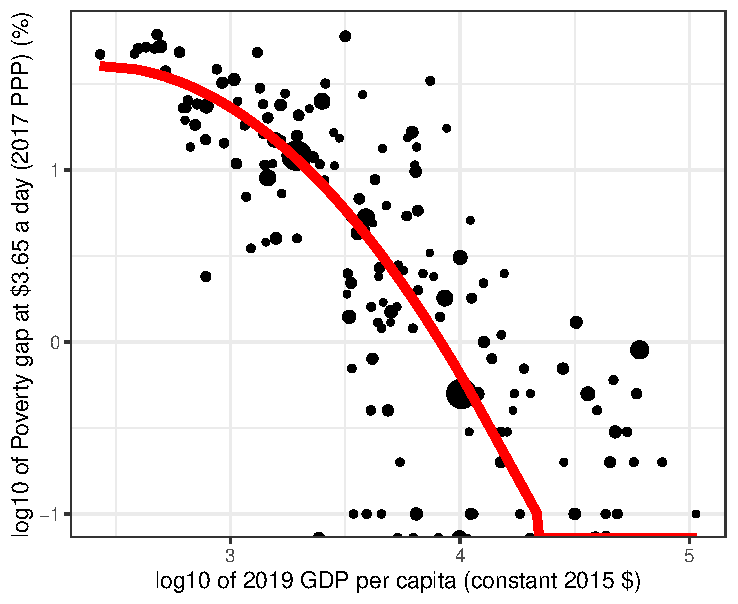
\includegraphics[width=.7\textwidth]{../figures/policies/poverty_gap4_gdp_quadratic_full}}  % poverty_gap_gdp
\end{figure}

\paragraph{Large transfers to Sub-Saharan Africa.} 
% I have removed the next three lines for clarity
% We define the share of total revenues allocated to a country as the product of its population and its \textit{statutory poverty gap}. We could simply define the statutory poverty gap as the poverty gap predicted by the regression just described, but this would imply allocating revenues to high-income countries. %, as some of them have a positive poverty gap. 
% Considering that high-income countries do not need extra resources to close their poverty gap, we set the statutory poverty gap at zero above an upper threshold defined as twice the global average GDP per capita. % (in PPP)
% To avoid threshold effects, we phase out the statutory poverty gap between a lower threshold set at the global average GDP per capita (of \$11,000 per year) and the upper threshold (see Figure \ref{fig:gap_GDP}). 
Table \ref{tab:allocation} (in Appendix) gives statistics on the revenues allocated to large countries (above 30 million inhabitants).\footnote{We do not show countries which are allocated zero revenues, or countries (like Poland) which are allocated less than 0.07\% of their GDP.} %India is the country that would receive the largest share of total revenues (19\%), followed by the DRC (11\%), Ethiopia (7\%), and Pakistan (5\%). 
Sub-Saharan Africa would receive 39\% of total revenues.  
Indeed, due to its high poverty gap, Sub-Saharan Africa would receive \$26 per month per capita, 3 times the global average, which would amount to 25\% of its GDP.
% 1-2-3: Indeed, due to its high poverty gap, Sub-Saharan Africa would receive \$28 per month per capita, 4 times the global average, which would amount to 25\% of its GDP. 
% (and up to 97\% in Madagascar) % Due to its very high poverty gap, Burundi would receive \$92 per month per capita, 22 times the global average, which would amount to 410\% of its GDP. 
% Low-income countries would receive 40\% of total revenues. Indeed, due to their high poverty gap, low-income countries would receive \$24 per month per capita, 5.5 times the global average, which would amount to 38\% of their GDP. 

\paragraph{In the long term, funding carbon removal.} 

After some years, stark poverty should be greatly reduced (if not totally eliminated). Given that poorer countries would receive more revenues, income inequality will diminish, especially between low-income countries and lower-middle-income countries. Therefore, as the policy goes on, the transfers would be less concentrated and would become more evenly spread out over low- and middle-income countries. As the poverty gap at \$3.65 a day would vanish at some point, the formula will need to change and allocate revenues based on a higher poverty line instead. In the second half of the century, the use of revenues could progressively shift from funding low-income countries to funding negative CO$_\text{2}$ emissions. Indeed, 5-15 GtCO$_\text{2}$ of carbon removal will be needed each year (through nature-based solutions like reforestation, bioenergy with carbon capture and storage, or direct air capture) to meet the climate target adopted in the Paris agreement \citep{ipcc_wgiii_2022}. The global wealth tax could provide an appropriate source of funding for tenders to remove predefined amounts of CO$_\text{2}$ from the atmosphere in line with the climate target (\citet{edenhofer_governance_2023} estimate the funding need at 0.3-3\% of world GDP in the second half of the century). 

\section{Support}\label{sec:support}

\paragraph{Near consensus for a global wealth tax.} \citet{fabre_international_2023} run representative surveys in 20 countries, on about 2,000 respondents per country. They ask the support for
``a tax on all millionaires in dollars around the world to finance low-income countries that comply with international standards regarding climate action [which] would finance infrastructure and public services such as access to drinking water, healthcare, and education'', in a 5-Likert scale from \textit{strongly oppose} to \textit{strongly support}. There is absolute majority support in each country, from 53\% in the U.S. to 86\% in China. Figure \ref{fig:support} shows that the relative support (excluding \textit{Indifferent} answers) ranges from 72\% in Denmark to 98\% in China. 


\citet{fabre_international_2023} also run complementary surveys on 2,000 Americans and on 3,000 Europeans (representative of France, Germany, Spain and the UK). Asking almost the same question (the only difference being that the revenues are allocated to low-income countries \textit{unconditional} on their climate action), they find comparable levels of support. The global wealth tax obtains absolute majority support in each of the five Western countries, with a relative support ranging from 70\% in the U.S. to 90\% in Spain (Figure \ref{fig:global_tax}). %Respondents are also asked to imagine that a global wealth tax is inplace, and w

\paragraph{People want one third of tax revenues for low-income countries.} \citet{fabre_international_2023} also ask respondents what percentage of the global tax revenues should be pooled to finance low-income countries, if a global tax on wealth (in excess of \$5 million) were in place. In each country, at least 88\% of respondents answer a positive amount, with an overall average of 30\% (Germany) to 36\% (U.S., France) (Figure \ref{fig:global_share_mean}).

\begin{figure}[h!] 
    \caption[Support for a global wealth tax]{Support for a global wealth tax. \\
    ``Do you support or oppose a tax on millionaires of all countries to finance low-income countries? \\
    Such tax would finance infrastructure and public services such as access to drinking water, healthcare, and education.''}\label{fig:global_tax}
    \makebox[\textwidth][c]{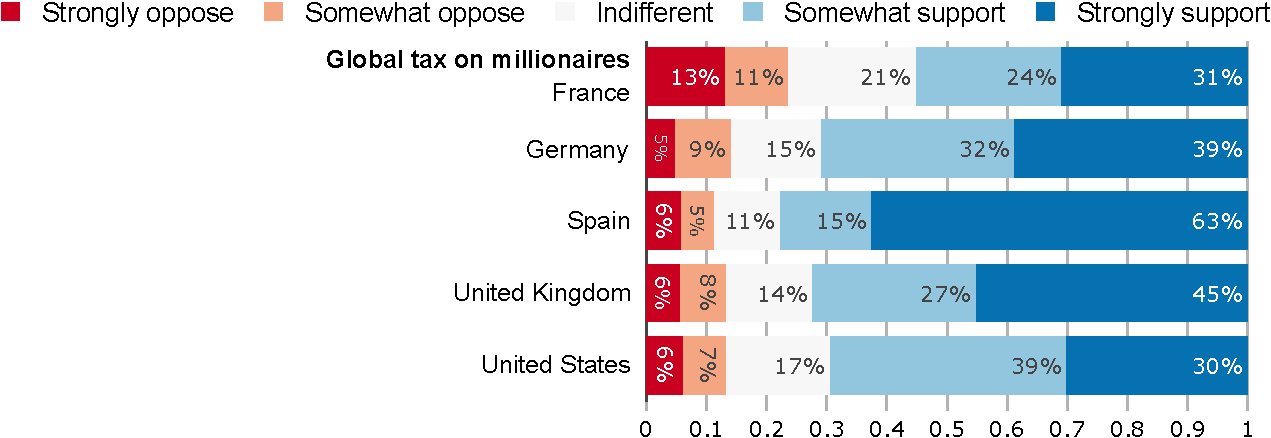
\includegraphics[width=\textwidth]{../figures/country_comparison/global_tax_support.pdf}} 
\end{figure}

\begin{figure}
    \centering 
    \caption[Preferred share of wealth tax for low-income countries]{Percent of global wealth tax that should finance low-income countries (\textit{mean}).} 
    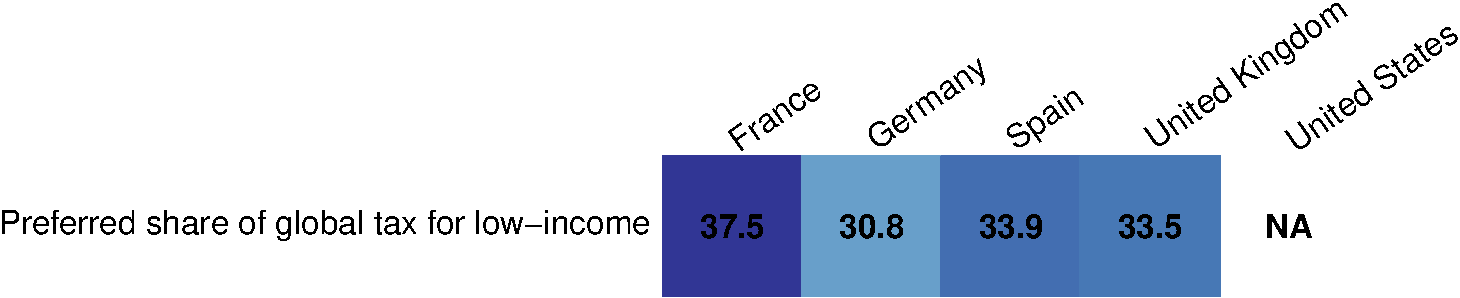
\includegraphics[width=1\textwidth]{../figures/country_comparison/global_tax_global_share_mean.pdf} \label{fig:global_share_mean}
\end{figure}

% \begin{figure}[h!]
%     \caption[Support for sharing half of global tax revenues with low-income countries]{Support for sharing half of global tax revenues with low-income countries, rather that each country retaining all the revenues it collects (in percent). (Question \ref{q:global_tax_sharing})}\label{fig:global_tax_sharing}
%     \makebox[\textwidth][c]{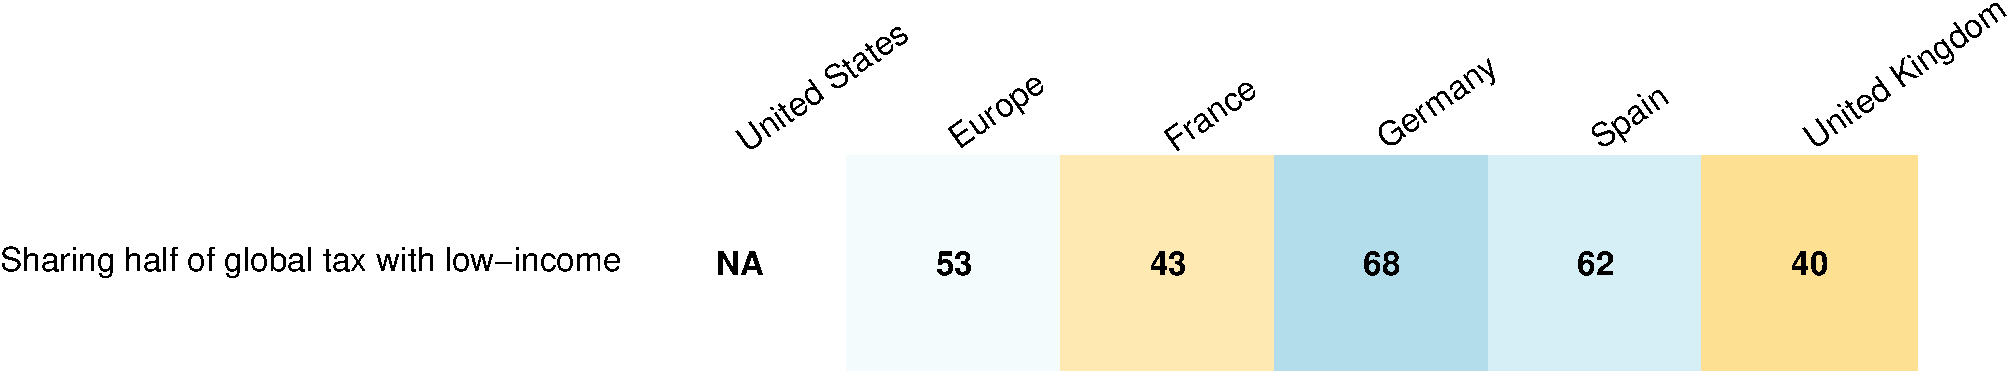
\includegraphics[width=\textwidth]{../figures/country_comparison/global_tax_sharing_positive.pdf}} 
% \end{figure}


\paragraph{A platform is preferred when it includes a global wealth tax.} \citet{fabre_international_2023} make people choose between two random platforms. In Europe, respondents are prompted to imagine that a left- or center-left coalition will win the next election and are asked what platform they would prefer that coalition to have campaigned on. In the U.S., the question is framed as a hypothetical duel in a Democratic primary, and asked only to non-Republicans. A policy (or an absence of policy) is randomly drawn for each platform in each of five categories: \textit{economic issues}, \textit{societal issues}, \textit{climate policy}, \textit{tax system}, \textit{foreign policy} (Figure \ref{fig:ca_r}). 
A platform that includes a global tax on millionaires rather that no foreign policy is 5 to 13 percentage points (p.p.) more likely to be preferred in all countries (the effect is significant and at least 9 p.p. in all countries but Spain). 
% A platform that includes a global tax on millionaires rather that no foreign policy is 9 to 13 percentage points (p.p.) more likely to be preferred in all countries but Spain (not significant, at +5 p.p.). 
These effects are large, and not far from the effects of the policies most influential on the platforms, which range between 15 and 18 p.p. in most countries (and 27 p.p. in Spain) and all relate to improved public services (in particular healthcare, housing and education). 

\begin{figure}[b!] 
    \caption[Preferences for various policies in political platforms in the UK]{Political preferences in the UK. \\ Effects of the presence of a policy (rather than none from this domain) in a random platform on the likelihood that it is preferred to another random platform. (For the other countries, see \citealp{fabre_international_2023})}\label{fig:ca_r}
      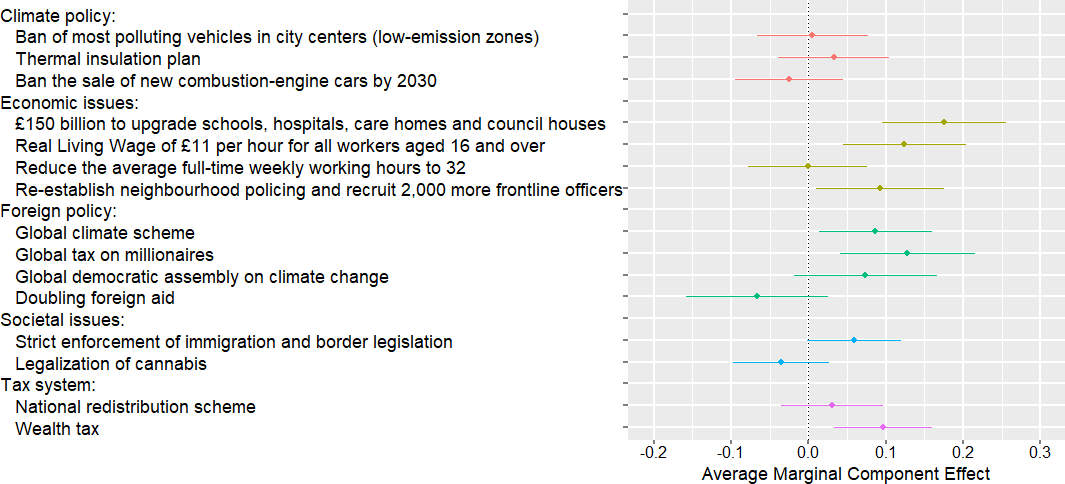
\includegraphics[width=\textwidth]{../figures/UK/ca_r.png}
    %\makebox[\textwidth][c]{} 
\end{figure}

% \begin{figure}
%   % Imagine that at the 2024 Democratic party presidential primaries, the two main candidates campaign with the following key policies in their platforms. \\ Which of these candidates do you prefer?

%   \caption{Conjoint analysis. Average Marginal Component Effects (relative to the baseline: an absence of policy of that category) of policies in the choice between two platforms, where policies in each platform are randomly drawn ($n$ = 6,000). In Eu, it is framed as two potential platforms of a left-wing coalition that would win the next elections; in the U.S., it is framed as a hypothetical duel in the 2024 Democratic primary and asked only to non-Republicans.}\label{fig:ca_r} 
%   \makebox[\textwidth][c]{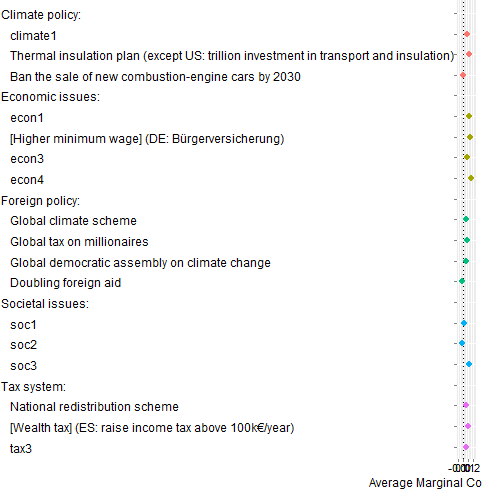
\includegraphics[width=\textwidth]{../figures/all/ca_r.png}}
% \end{figure}

\paragraph{A global wealth tax is one of the main priorities.} Each respondent is then asked to allocate 100 points among six policies picked at random (among the policies used in the previous question), with the instruction that ``the more you give points to a policy, the more you support it''. For each policy presented, the average support is thus 16.67 points.  The global tax on millionaires ranks at worst in fifth position (out of 15 or 17) in every country, and receives an average number of points from 18.3 (Spain) to 22.9 (Germany). 
In Germany, the global tax on millionaires is the most prioritized policy. In other countries, the most prioritized policies relate to improved public services (in particular healthcare, housing and education) and are thus complementary to a wealth tax, which can finance them.
\quad \\ \quad 

\textit{We are here to feed the public debate on global redistribution. We welcome counter-proposals, criticisms and suggestions concerning our policy brief (including pull requests). Feel free to engage the discussion on \href{https://github.com/bixiou/global_tax_attitudes/issues}{github}. }

\begin{figure}[h!] % TODO add red rectangle on tax, same for ca_r
  \caption[Mean prioritization of policies]{Mean prioritization of policies. \\Mean number of points allocated policies to express intensity of support (among six policies chosen at random). Blue color means that the policy has been awarded more points than the average policy.}\label{fig:points}
  \makebox[\textwidth][c]{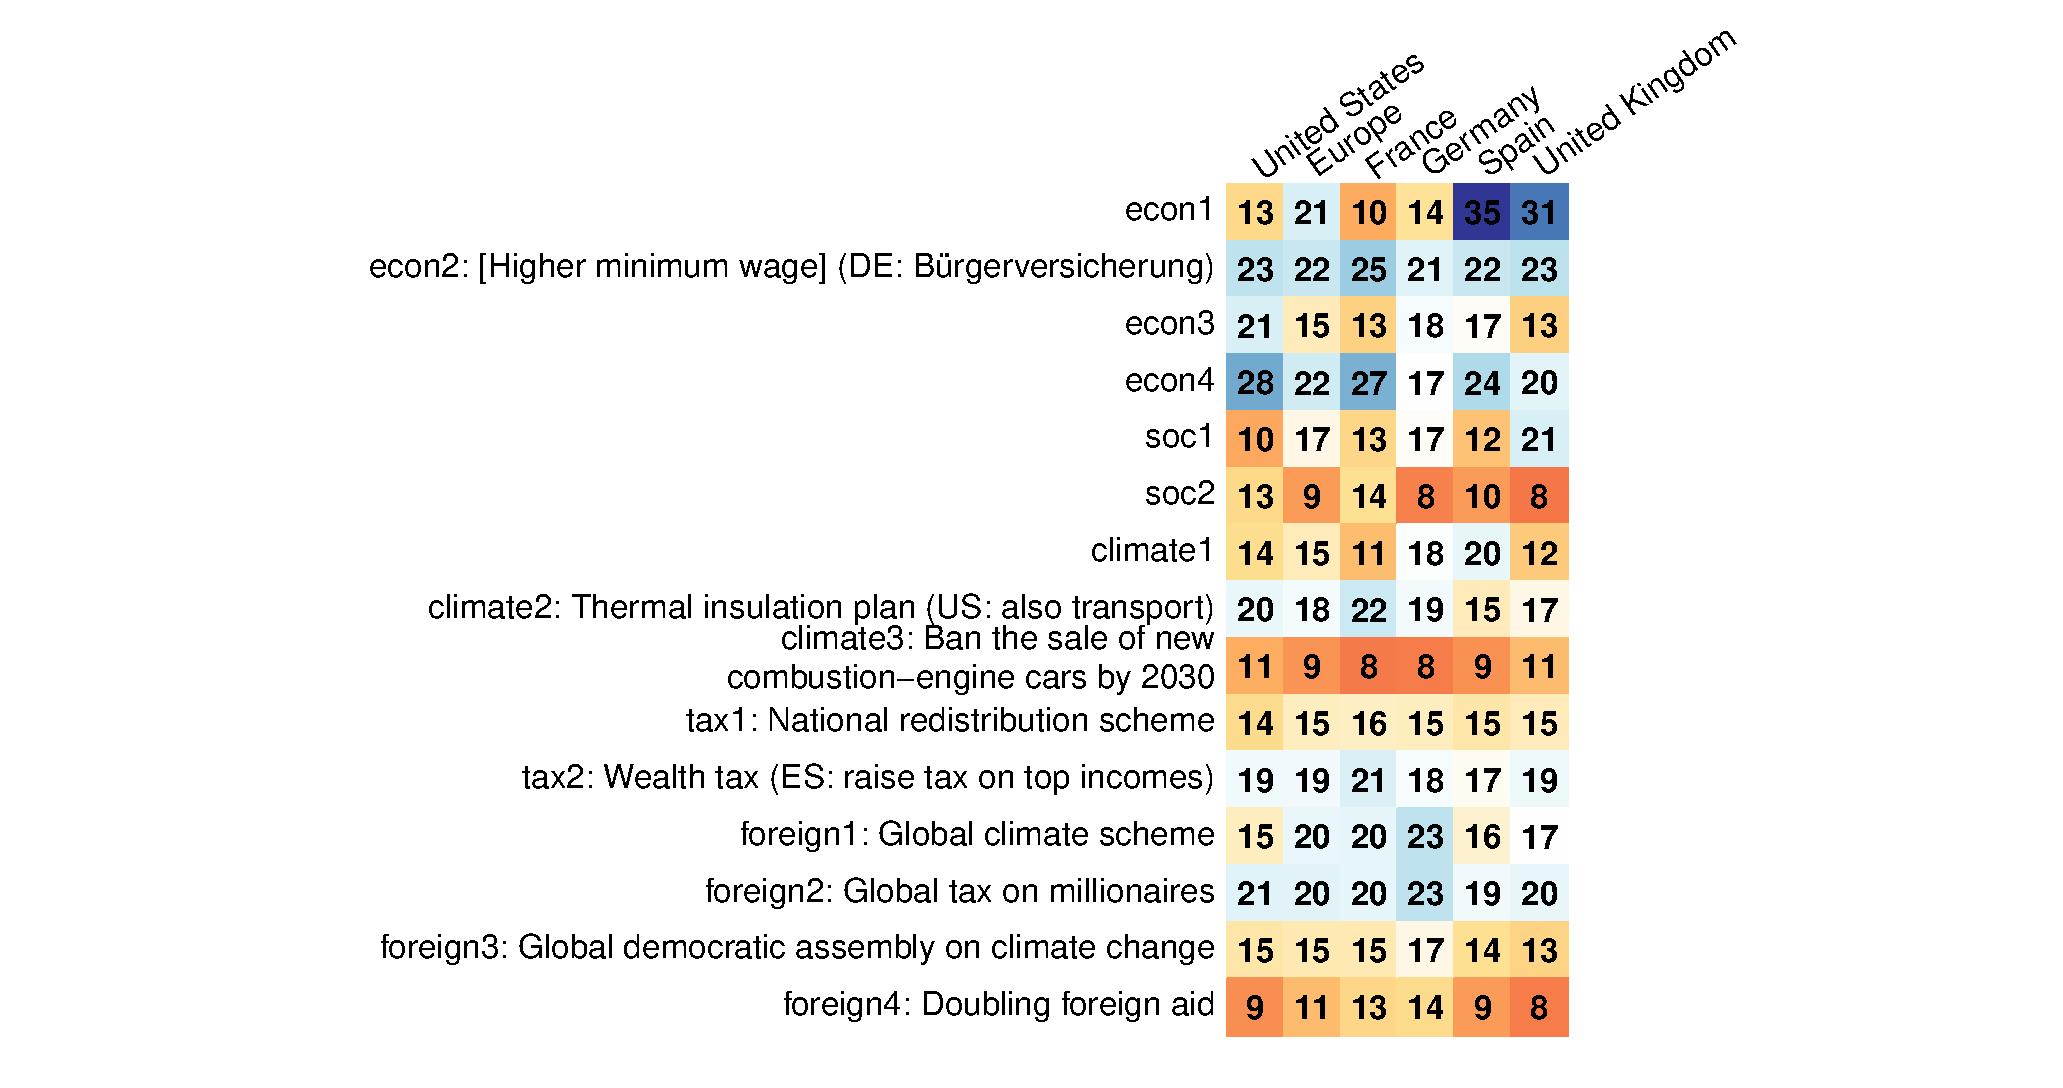
\includegraphics[width=\textwidth]{../figures/country_comparison/points_mean.pdf}} 
\end{figure}
% TODO! update figure so that it is "global tax on millionaires financing..."

% \section*{Allocation of revenues between countries}
\clearpage
% \begin{multicols}{2}
%     \setbox\ltmcbox\vbox{
%     \makeatletter\col@number\@ne
        
\begin{longtable}[t]{lrrrr}
\caption{\label{tab:allocation}Allocation of the global wealth tax revenues.}\\
\toprule
  & \makecell{Revenues\\over GDP\\(in percent)} & \makecell{Revenues\\per capita\\(in \$ per month)} & \makecell{Revenues per capita\\over average\\revenues p.c.} & \makecell{Global\\share of\\revenues}\\
\midrule
Madagascar & 112.20 & 45 & 4.65 & 1.76\\
DRC & 105.95 & 44 & 4.54 & 5.79\\
Afghanistan & 79.10 & 39 & 4.00 & 2.11\\
Mozambique & 75.43 & 38 & 3.92 & 1.66\\
Yemen & 57.32 & 34 & 3.48 & 1.50\\
Ethiopia & 47.05 & 31 & 3.20 & 5.05\\
Uganda & 35.51 & 27 & 2.83 & 1.72\\
Tanzania & 28.84 & 25 & 2.59 & 2.18\\
Nepal & 27.73 & 25 & 2.55 & 0.98\\
Pakistan & 15.98 & 19 & 2.01 & 6.03\\
Bangladesh & 14.13 & 18 & 1.91 & 4.11\\
Myanmar & 13.82 & 18 & 1.89 & 1.29\\
Kenya & 12.72 & 18 & 1.82 & 1.25\\
India & 9.60 & 16 & 1.61 & 28.76\\
Sudan & 9.53 & 15 & 1.61 & 0.97\\
Ghana & 9.26 & 15 & 1.59 & 0.68\\
Ukraine & 6.49 & 13 & 1.36 & 0.63\\
Nigeria & 6.13 & 13 & 1.33 & 3.71\\
Angola & 5.69 & 12 & 1.26 & 0.58\\
Uzbekistan & 3.06 & 8 & 0.84 & 0.37\\
Vietnam & 2.72 & 7 & 0.77 & 0.95\\
Morocco & 2.56 & 7 & 0.74 & 0.35\\
Philippines & 2.09 & 6 & 0.65 & 0.95\\
Egypt & 1.81 & 6 & 0.59 & 0.83\\
Indonesia & 1.64 & 5 & 0.55 & 1.92\\
Algeria & 1.35 & 5 & 0.49 & 0.28\\
Iraq & 0.85 & 3 & 0.36 & 0.20\\
Iran & 0.77 & 3 & 0.33 & 0.37\\
South Africa & 0.41 & 2 & 0.22 & 0.17\\
Colombia & 0.37 & 2 & 0.21 & 0.13\\
Thailand & 0.36 & 2 & 0.20 & 0.18\\
Peru & 0.35 & 2 & 0.20 & 0.08\\
Brazil & 0.15 & 1 & 0.11 & 0.31\\
Russia & 0.10 & 1 & 0.09 & 0.15\\
Mexico & 0.10 & 1 & 0.08 & 0.13\\
China & 0.09 & 1 & 0.08 & 1.46\\
Malaysia & 0.07 & 1 & 0.07 & 0.03\\
\bottomrule
\end{longtable}
%     \unskip
%     \unpenalty
%     \unpenalty}
%     \unvbox\ltmcbox
% \end{multicols}

\clearpage
\renewcommand{\url}[1]{\href{#1}{Link}} % NCCcomment
\bibliographystyle{plainnaturl_clean} % NCCcomment
\bibliography{global_tax_attitudes}

\end{document}